\section{Robot Model}
As mentioned in the problem setup section, we only use a gripper without the arm to increase computation speed. This setup obliviates the need for inverse kinematics calculation for each joint of a whole robotics arm. Although we deviate from the real-world setting by excluding the arm, Breyer et al. showed that the model learned without the entire kinematic chain can still perform successfully on the real-world robot \cite{Breyer2018}. This success stems from the small working setup comprises only 10cm to 10cm area and the limited translation and yaw rotation motions, 3cm and 15cm accordingly.

We noticed that in Breyer et al. setting, because of the narrow gripper width of the robot model (ABB Yumi), it could not perform at its maximum potential \ref{fig:breyer}. Thus, we selected a gripper (WSG50) that has a broader gripper opening \ref{fig:ourmodel}. As a result, we could use the object models without scaling. Whereas Breyer et al. scaled-down the object \(70\%\) smaller.


\begin{figure}

    \begin{subfigure}{0.35\textwidth}
      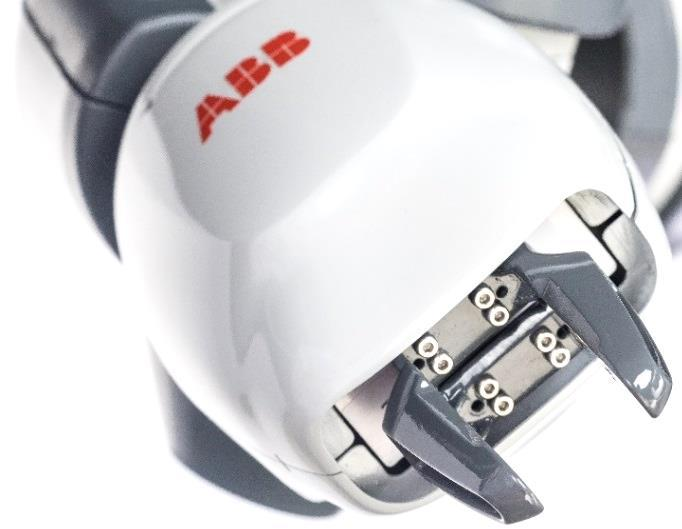
\includegraphics[width=\linewidth]{figures/abbyumi.jpg}
      \caption{ABB Yumi gripper model} \label{fig:ABBYUMI}
    \end{subfigure}%
    \hspace*{\fill}   % maximize separation between the subfigures
    \begin{subfigure}{0.35\textwidth}
      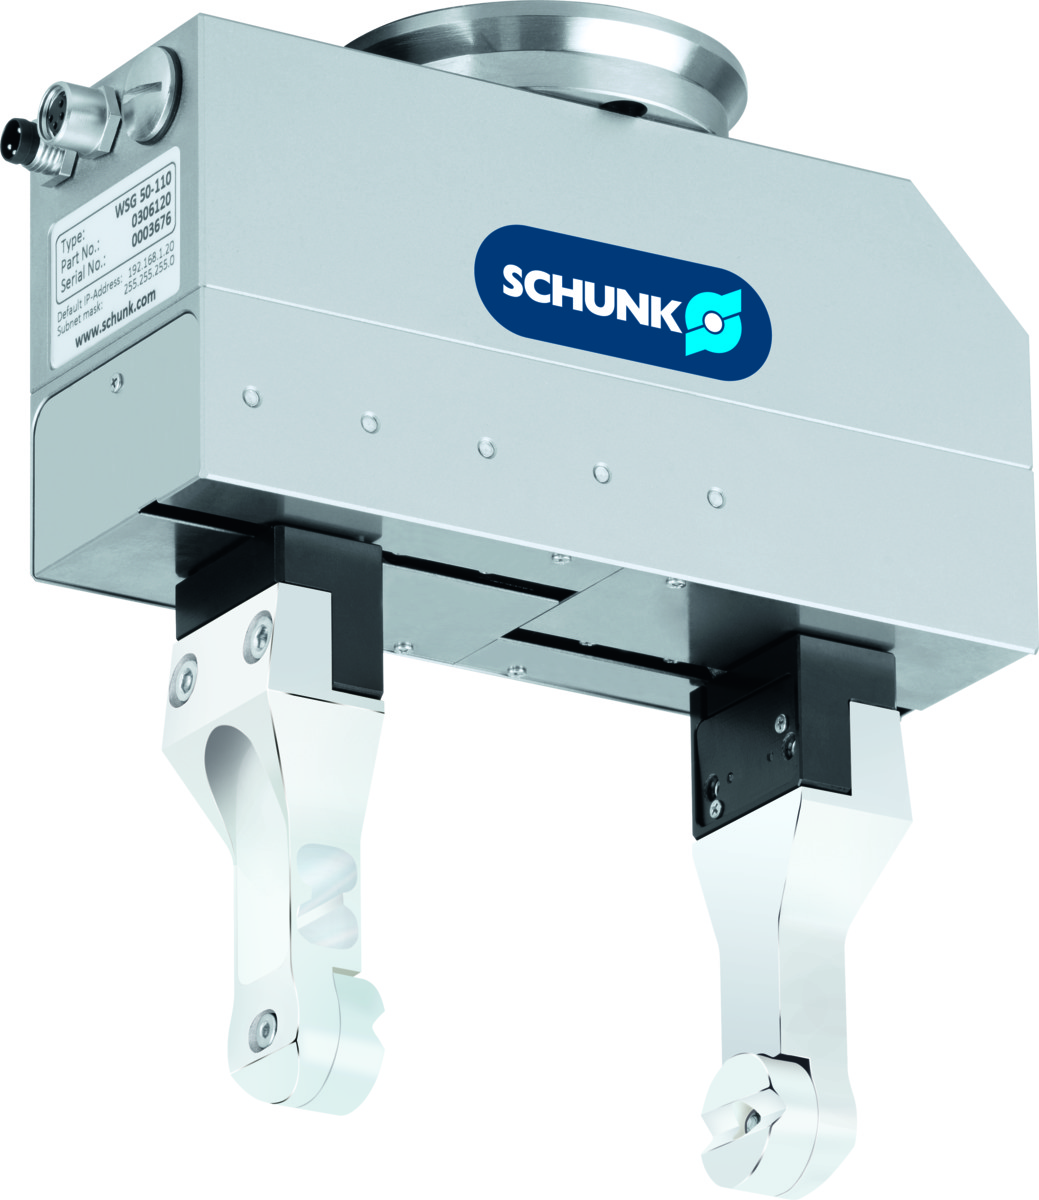
\includegraphics[width=\linewidth]{figures/wsg50.jpg}
      \caption{WSG50 gripper model} \label{fig:WSG50}
    \end{subfigure}%
    \hspace*{\fill}   % maximize separation between the subfigures


\caption{ Real images of gripper models   \label{fig:robots}}
\end{figure}

\begin{figure}

    \begin{subfigure}{0.49\textwidth}
      \includegraphics[width=\linewidth]{figures/breyerModel.png}
      \caption{ABB Yumi gripper used in Breyer et al.} \label{fig:breyer}
    \end{subfigure}%
    \hspace*{\fill}   % maximize separation between the subfigures
    \begin{subfigure}{0.49\textwidth}
      \includegraphics[width=\linewidth]{figures/ourModel.png}
      \caption{WSG50 gripper used in our work} \label{fig:ourmodel}
    \end{subfigure}%
    \hspace*{\fill}   % maximize separation between the subfigures


\caption{ Different robot models \label{fig:robots}}
\end{figure}